\documentclass[11pt, a4paper]{scrartcl}

\title{Julia Installationsanleitung für Windows}
\author{}
\date{}

\usepackage{listings}
\usepackage{jlcode}
\usepackage{color}
\usepackage{hyperref}
\usepackage{graphicx}

\definecolor{dkgreen}{rgb}{0,0.6,0}
\definecolor{gray}{rgb}{0.5,0.5,0.5}
\definecolor{mauve}{rgb}{0.58,0,0.82}

\lstset{
	language=Julia,
%	frame=tb,
	aboveskip=3mm,
	belowskip=3mm,
	showstringspaces=false,
	columns=flexible,
	basicstyle={\small\ttfamily},
	numbers=none,
	numberstyle=\tiny\color{gray},
	keywordstyle=\color{blue},
	commentstyle=\color{dkgreen},
	stringstyle=\color{mauve},
	breaklines=true,
	breakatwhitespace=true,
	tabsize=3
}



\begin{document}
	\maketitle
	
	\section{Julia herunterladen und installieren}
%	\href{http://julialang.org}{julialang.org}
%	\url{http://julialang.org}
	Öffnen Sie die Webseite \url{https://julialang.org/downloads/} in ihrem Browser (Sie können auf alle Links in dieser PDF klicken und der Browser sollte sich automatisch öffnen). Klicken Sie dort auf den ersten Link mit der Bezeichnung \texttt{64-bit}, um die Julia Installationsdatei herunterzuladen.
	
	\begin{figure}[h!]
		\centering
		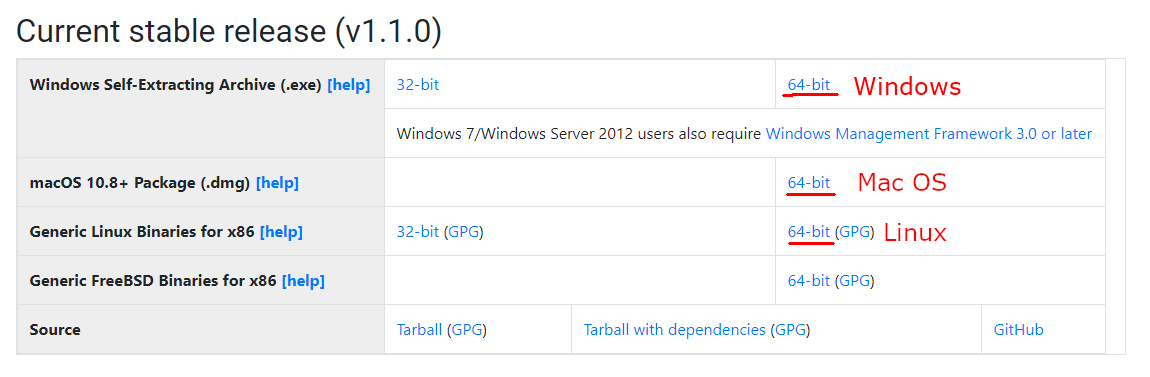
\includegraphics[width=\textwidth]{imgs/download.png}
	\end{figure}

	Führen Sie die heruntergeladene Datei aus. Es sollte nach einem Ladebalken folgendes Fenster erscheinen (eventuell ist der Dialog bei Ihnen auf Deutsch):
	
	\begin{figure}[h!]
		\centering
		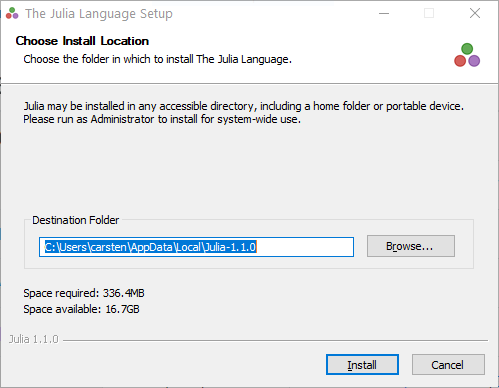
\includegraphics[width=0.5\textwidth]{imgs/install.png}
	\end{figure}

	Klicken Sie auf \texttt{Install}, um Julia zu installieren. Nach Abschluss der Installation erscheint folgender Dialog: 
	

	\begin{figure}[h!]
	\centering
	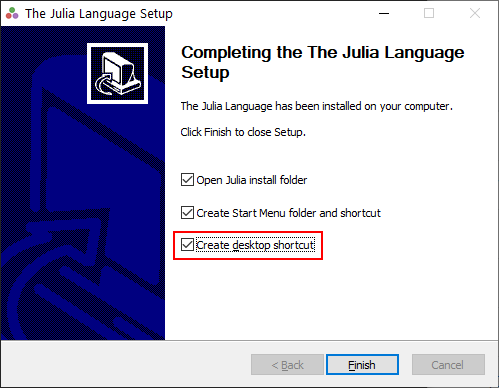
\includegraphics[width=0.5\textwidth]{imgs/install_finish.png}
	\end{figure}

	Setzen Sie beim dritten Auswahlpunkt \texttt{Create desktop shortcut} einen Haken, damit eine Julia Verknüpfung auf dem Desktop erstellt wird. Schließen Sie die Installation mit einem Klick auf \texttt{Finish} ab.
	
	\newpage
	\section{IJulia und Jupyter installieren}
	
	Neben der Programmiersprache Julia selbst, benötigen wir noch IJulia, um Julia bequem im Browser in sogenannten Jupyter Notebooks verwenden zu können. Im folgenden wollen wir IJulia installieren.

	Starten Sie Julia durch einen Doppelklick auf das Julia Logo auf dem Desktop (oder per Startmenü). Führen Sie folgenden Befehl aus, indem Sie ihn abtippen (bitte nicht kopieren und einfügen) und mit der \texttt{Enter}-Taste bestätigen.
	
	\begin{lstlisting}
		using Pkg; Pkg.add("IJulia");
	\end{lstlisting}

	Insgesamt sollten Sie folgende Ausgabe erhalten (die Dateipfade können abweichen):
	
	\begin{figure}[h!]
	\centering
	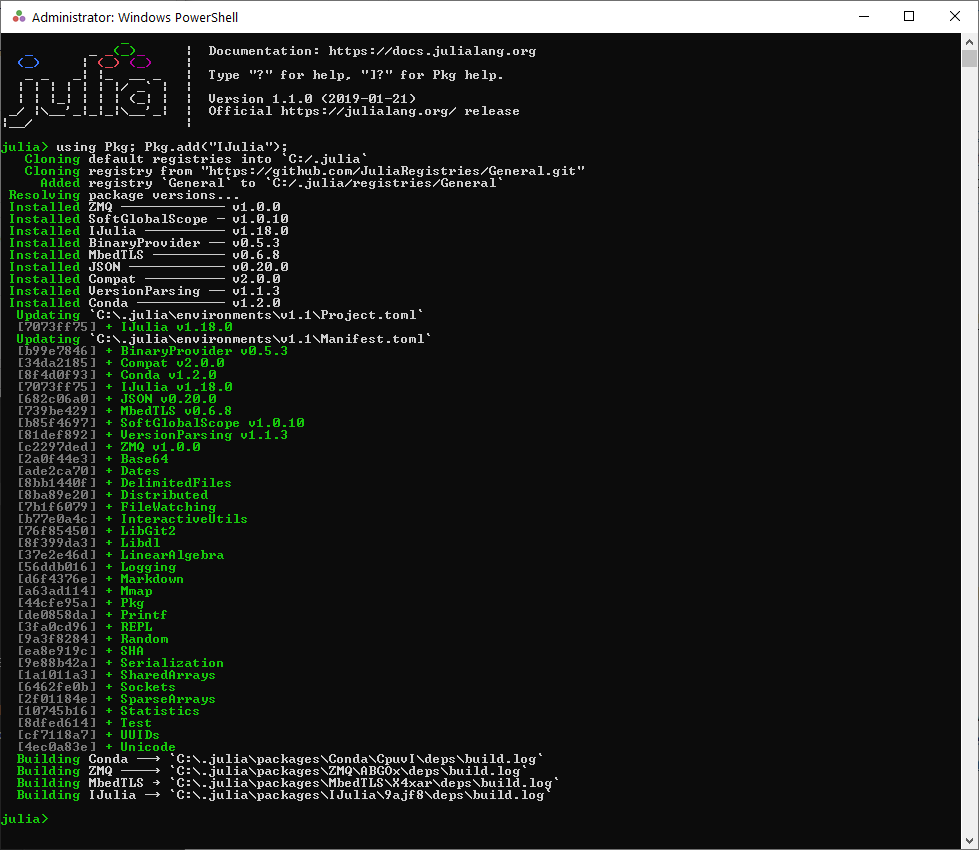
\includegraphics[width=0.9\textwidth]{imgs/IJulia_install.png}
	\end{figure}

	IJulia ist nun erfolgreich installiert. Führen Sie nun den Befehl
	
	\begin{lstlisting}
	using IJulia
	\end{lstlisting}
	
	aus. Julia stellt fest, das Jupyter noch nicht vorhanden ist, und fragt uns, ob wir es installieren wollen:
	
	\begin{figure}[h!]
	\centering
	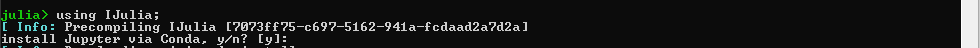
\includegraphics[width=0.9\textwidth]{imgs/Jupyter_install.png}
	\end{figure}

	Dies bestätigen wir durch Drücken der \texttt{Enter}-Taste. Die Installation von Jupyter kann eventuell einige Minuten dauern. Die Installation ist abgeschlossen, wenn sie wieder das grüne \texttt{julia>} Zeichen am Anfang der Zeile sehen.
	
	\section{IJulia und Jupyter starten}
	
	Um Jupyter Notebooks erstellen oder öffnen zu können, müssen wir immer zuerst Julia und dann den Jupyter Server starten. Dazu führen wir den folgenden Befehl in der Julia Konsole aus (öffnen Sie diese per Doppelklick auf das Julia Logo auf dem Desktop, falls sie nicht bereits offen ist):
	
	\begin{lstlisting}
	using IJulia; notebook()
	\end{lstlisting}
	
	Es sollte sich der Browser öffnen und das Jupyter Notebook Interface erscheinen (Ordner, Dateien und Sprache können abweichen):
	
	\begin{figure}[h!]
	\centering
	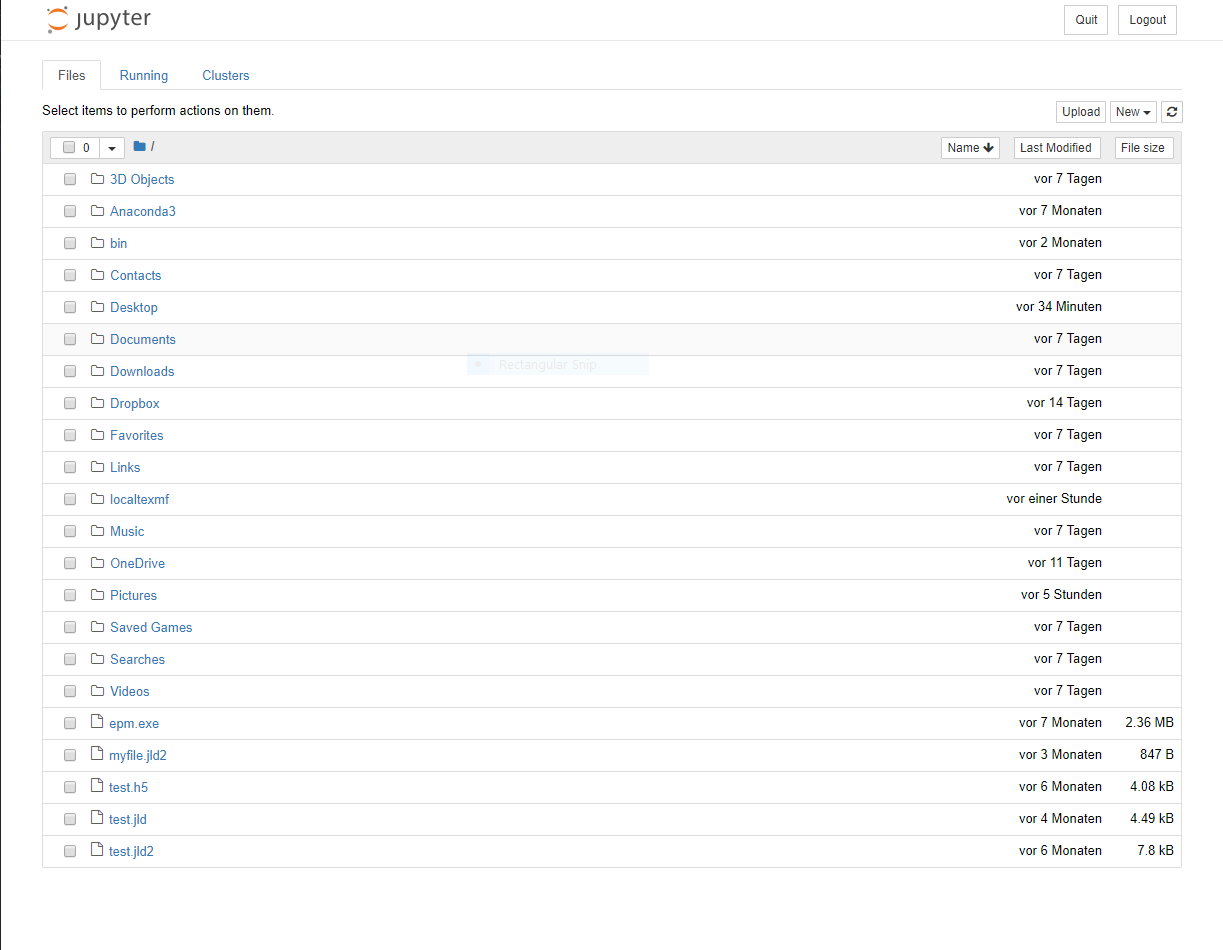
\includegraphics[width=0.7\textwidth]{imgs/jupyter.png}
	\caption{Die Startseite des Jupyter Interfaces. \label{fig:jupyter}}
	\end{figure}
	
	Der Server läuft solange die Julia Konsole im Hintergrund geöffnet ist. Sobald wir diese schließen wird der Server gestoppt.
	
	\newpage
	\section{Einfacher Test das alles funktioniert}
	
	Klicken Sie im Jupyter Interface (Fig. \ref{fig:jupyter}) rechts oben auf den Button \texttt{New} und klicken Sie danach im sich öffnenden Kontextmenü auf den Eintrag \texttt{Julia 1.1.0}. Es sollte sich nun ein frisches Jupyter Notebook öffnen:
	
	\begin{figure}[h!]
	\centering
	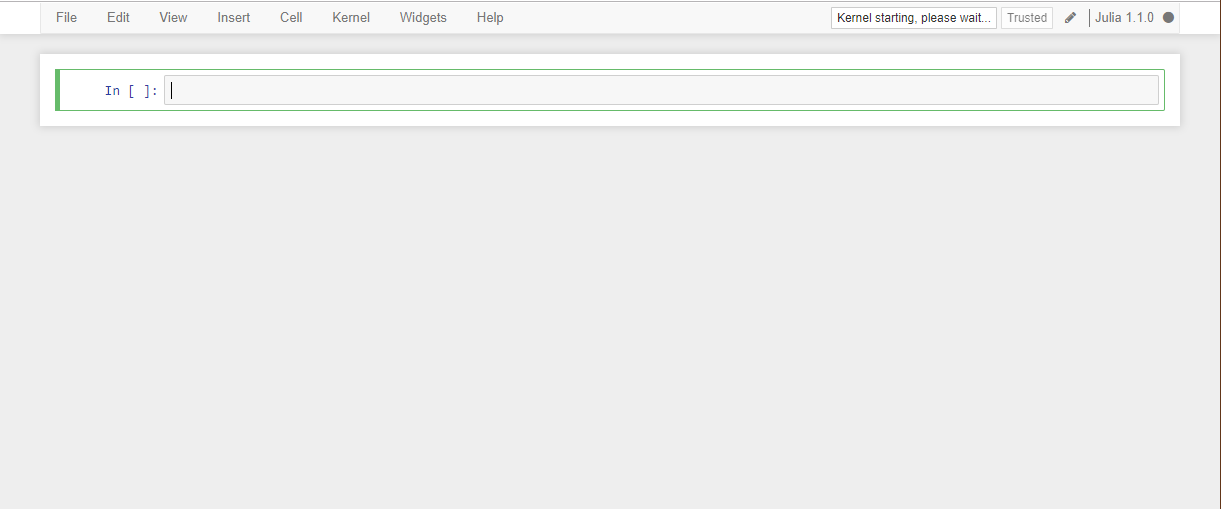
\includegraphics[width=0.9\textwidth]{imgs/jupyter_notebook.png}
	\end{figure}

	Klicken Sie in die erste (und einzige) Zelle des Notebooks und geben Sie dort
	
	\begin{lstlisting}
	3+3
	\end{lstlisting}
	ein. Führen Sie die Zelle per \texttt{SHIFT + ENTER} aus (gleichzeitiges Drücken der \texttt{SHIFT} bzw. \texttt{UMSCHALT} und der \texttt{ENTER} Taste). Es sollte das Ergebnis \texttt{6} erscheinen:

	\begin{figure}[h!]
	\centering
	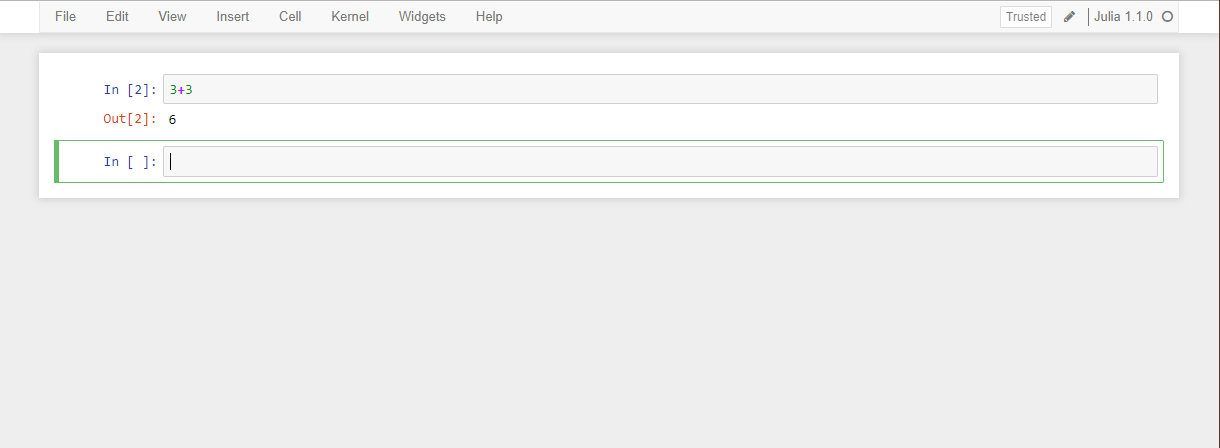
\includegraphics[width=0.9\textwidth]{imgs/jupyter_notebook_test.png}
	\end{figure}	

	Die Installation von Julia, IJulia und Jupyter war also erfolgreich!
	
\end{document}